\documentclass[11pt,a4paper]{article}
\usepackage[margin=2.3cm]{geometry}
\usepackage{amsmath,amssymb,bm}
\usepackage{siunitx}
\usepackage{booktabs}
\usepackage{graphicx}
\usepackage{tikz}
\usetikzlibrary{arrows.meta,calc,positioning,patterns}
\usepackage{pgfplots}
\pgfplotsset{compat=1.17}
\usepackage{enumitem}
\usepackage{float}
\tikzset{capt/.style={text width=5.2cm,align=center}}
\usepackage[colorlinks=true,linkcolor=blue!60!black,urlcolor=blue!60!black]{hyperref}
\usepackage{fancyhdr}
\usepackage{tcolorbox}
\tcbuselibrary{skins,breakable}
\sisetup{per-mode=symbol,detect-all}
\DeclareSIUnit{\MParm}{MPa\,\ensuremath{\sqrt{\text{m}}}}

\newtcolorbox{keybox}[1]{title={#1},colback=blue!4,colframe=blue!50!black,fonttitle=\bfseries,breakable}
\newtcolorbox{examplebox}[1]{title={#1},colback=green!4,colframe=green!40!black,fonttitle=\bfseries,breakable}
\newtcolorbox{aerobox}[1]{title={#1},colback=orange!5,colframe=orange!60!black,fonttitle=\bfseries,breakable}

\pagestyle{fancy}
\fancyhf{}
\lhead{
\includegraphics[height=0.6cm]{logos/itu_logo_laci.pdf}\ \ UCK 364E Design of Machine Elements}
\setlength{\headheight}{20pt}
\rhead{Lecture 4 -- Notes}
\cfoot{\thepage}

\title{\textbf{UCK 364E Design of Machine Elements}\\[4pt]
\Large Lecture 4: Fatigue under Combined and Variable Loading\\[2pt]
\large Multiaxial stress, equivalent-stress and critical-plane methods, rainflow counting, spectrum fatigue}
\author{Prof.\ Dr.\ Onur Tunçer\\ Department of Aeronautical Engineering, Istanbul Technical University}
\date{Fall 2026}

\begin{document}
\maketitle

\section*{Learning objectives}
By the end of this lecture you should be able to
\begin{enumerate}[nosep]
  \item distinguish proportional from non-proportional multiaxial loading, and explain why the distinction matters for fatigue but not for static yielding;
  \item apply the von Mises equivalent-stress method to a combined-loading fatigue problem, and state the two things it gets wrong;
  \item use the Gough ellipse and the DE--Goodman shaft equations, and compute a safety factor for a shaft in combined bending and torsion;
  \item explain what a critical-plane method does and when it is required;
  \item carry out rainflow counting by hand on a short stress history, and explain why it is the only counting method consistent with the material's memory;
  \item accumulate damage over a counted spectrum with Palmgren--Miner, identify which cycles dominate, and apply a scatter factor;
  \item describe how an aircraft load spectrum is assembled from GAG, gust, manoeuvre and ground loads, and what a flight-by-flight sequence is for;
  \item state how S--N data scatter is treated statistically (ASTM E739) and why the design curve is not the mean curve.
\end{enumerate}

\section{Why this lecture exists}

Every worked example so far has been uniaxial: a skin in hoop tension, a lug in bearing, a rod in axial load. Almost no real machine element is loaded that way.

\begin{center}\small
\begin{tabular}{@{}lll@{}}
\toprule
Element & Stress state & Phasing \\
\midrule
Rotating shaft with a pulley & bending (alternating) $+$ torsion (steady) & fixed phase \\
Landing-gear axle & bending from vertical load $+$ torsion from braking & \emph{independent} \\
Lug in a control linkage & axial $+$ secondary bending from eccentricity & in phase \\
Welded cluster joint & force $+$ moment on the weld group & in phase \\
Pressurised fuselage & hoop $+$ longitudinal $+$ local bending at the lap & in phase \\
Propeller blade root & centrifugal (steady) $+$ 1P bending (alternating) $+$ torsion & mixed \\
Bolt in a flanged joint & preload tension (steady) $+$ cyclic tension $+$ bending & in phase \\
\bottomrule
\end{tabular}
\end{center}

Lecture 2 gave us S--N and $\varepsilon$--N for a single alternating stress; Lecture 3 gave us crack growth for a single $\Delta K$. This lecture supplies the two bridges needed before either is usable on a real part:

\begin{enumerate}[nosep]
  \item \textbf{From a multiaxial stress state to one equivalent alternating stress.}
  \item \textbf{From a messy measured load history to a counted set of cycles.}
\end{enumerate}

\begin{keybox}{The two bridges}
Without the first, you do not know \emph{what stress} to look up on the S--N curve.\\
Without the second, you do not know \emph{how many cycles} of it there are.
\end{keybox}

\section{Proportional and non-proportional loading}

Consider a point carrying a normal stress $\sigma(t)$ and a shear stress $\tau(t)$. Plot the loading path in the $\sigma$ versus $\sqrt3\,\tau$ plane over one cycle.

\begin{itemize}[nosep]
  \item If $\sigma$ and $\tau$ vary \emph{in a fixed ratio} --- both driven by the same load, or by loads that rise and fall together --- the path is a \textbf{straight line through the origin}. The principal directions do not rotate. This is \textbf{proportional} (or in-phase) loading.
  \item If they vary independently --- a landing-gear axle whose vertical load and brake torque have nothing to do with each other --- the path is an \textbf{ellipse or a loop}. The principal directions rotate during the cycle. This is \textbf{non-proportional} loading.
\end{itemize}

\begin{figure}[H]\centering
\begin{tikzpicture}[scale=1.0,>=Stealth,font=\scriptsize]
\begin{scope}
\draw[->] (-2.6,0) -- (2.8,0) node[right] {$\sigma$};
\draw[->] (0,-2.3) -- (0,2.5) node[above] {$\sqrt3\,\tau$};
\draw[very thick,blue!60!black] (-2.0,-1.3) -- (2.0,1.3);
\fill[blue!60!black] (2.0,1.3) circle (1.6pt); \fill[blue!60!black] (-2.0,-1.3) circle (1.6pt);
\node[anchor=north,align=center] at (0,-2.7) {\textbf{proportional}\\ principal directions fixed};
\end{scope}
\begin{scope}[xshift=7.2cm]
\draw[->] (-2.6,0) -- (2.8,0) node[right] {$\sigma$};
\draw[->] (0,-2.3) -- (0,2.5) node[above] {$\sqrt3\,\tau$};
\draw[very thick,red!70!black] (0,0) ellipse (2.0 and 1.3);
\draw[->,red!70!black,very thick] (2.0,0) arc (0:40:2.0 and 1.3);
\node[anchor=north,align=center] at (0,-2.7) {\textbf{non-proportional}\\ principal directions rotate};
\end{scope}
\end{tikzpicture}
\caption{Loading paths over one cycle. Both states may have identical von Mises amplitudes, and identical static margins --- but under cyclic loading the non-proportional case can have a life an order of magnitude shorter, because the rotating principal directions activate slip on more planes and the material hardens additionally.}
\label{fig:prop}
\end{figure}

\begin{keybox}{Why static analysis does not care, but fatigue does}
For a \emph{static} check you evaluate von Mises at the worst instant and compare with $S_y$: the path taken to get there is irrelevant. For \emph{fatigue} the whole path matters, because damage accumulates by cyclic slip on particular crystallographic planes. A rotating principal direction sweeps the slip activity around, hardens the material by an extra 20--40\%, and --- counter-intuitively --- \emph{shortens} life, typically by a factor of 2--10 for 90$^\circ$ out-of-phase loading.
\end{keybox}

\section{Equivalent-stress methods}

\subsection{The von Mises amplitude}
The practical engineering approach is to collapse the multiaxial state into a single equivalent alternating stress and a single equivalent mean stress, then use the Lecture~2 machinery unchanged. Compute the amplitude and mean of each stress component separately, then combine:
\begin{align}
  \sigma'_a&=\sqrt{\left(K_f\sigma_{a}\right)^{2}+3\left(K_{fs}\tau_{a}\right)^{2}}, \label{eq:vma}\\
  \sigma'_m&=\sqrt{\left(K_f\sigma_{m}\right)^{2}+3\left(K_{fs}\tau_{m}\right)^{2}}, \label{eq:vmm}
\end{align}
with separate fatigue notch factors for normal and shear stress ($K_{fs}$ uses $K_{ts}$ for the same geometry). These then go into any of the Lecture~2 mean-stress criteria; with Goodman,
\begin{equation}
  \frac{1}{n}=\frac{\sigma'_a}{S_e}+\frac{\sigma'_m}{S_{ut}} .
  \label{eq:degoodman}
\end{equation}
This is the \textbf{DE--Goodman} method (DE for distortion energy), and for a solid round shaft of diameter $d$ carrying bending $M$ and torque $T$ it can be written directly in terms of the loads:
\begin{equation}
  \frac{1}{n}=\frac{16}{\pi d^{3}}\left\{
  \frac{\left[4(K_fM_a)^{2}+3(K_{fs}T_a)^{2}\right]^{1/2}}{S_e}
  +\frac{\left[4(K_fM_m)^{2}+3(K_{fs}T_m)^{2}\right]^{1/2}}{S_{ut}}\right\}.
  \label{eq:shaft}
\end{equation}
Rearranged for the unknown diameter, this is the shaft-sizing equation you will use repeatedly.

\begin{aerobox}{Two things the von Mises amplitude gets wrong}
\textbf{1. It is a positive quantity and therefore blind to sign.} Equations \eqref{eq:vma}--\eqref{eq:vmm} cannot distinguish tension from compression in the mean, which matters enormously for fatigue. The usual repair is to carry the sign of the dominant principal stress, or of the hydrostatic stress, into $\sigma'_m$ --- otherwise a beneficial \emph{compressive} mean is counted as damaging.

\medskip
\textbf{2. It assumes proportional loading.} The derivation collapses the history to amplitudes and means component by component, which silently discards the phase relationship. For non-proportional loading it is \emph{non-conservative}, sometimes badly so.
\end{aerobox}

\subsection{The Gough ellipse: combined bending and torsion}
Gough and Pollard tested shafts under combined bending and torsion and found that the fatigue limits lie on an ellipse:
\begin{equation}
  \left(\frac{\sigma_a}{S_e}\right)^{2}+\left(\frac{\tau_a}{S_{se}}\right)^{2}=1 ,
  \label{eq:gough}
\end{equation}
with $S_{se}\approx0.577\,S_e$ for ductile metals --- which makes Eq.~\eqref{eq:gough} identical to the von Mises criterion applied to amplitudes. For brittle and notched materials the data fit an ellipse-arc with $S_{se}/S_e$ nearer 0.8, and the design curve must be shifted accordingly.

\begin{figure}[H]\centering
\begin{tikzpicture}
\begin{axis}[width=10.4cm,height=5.4cm,xlabel={$\sigma_a/S_e$},ylabel={$\tau_a/S_{se}$},
 xmin=0,xmax=1.25,ymin=0,ymax=1.25,grid=both,grid style={gray!20},
 label style={font=\footnotesize},tick label style={font=\footnotesize},
 legend pos=south west,legend style={font=\scriptsize},legend cell align=left]
\addplot[very thick,blue!60!black,domain=0:1,samples=120]{sqrt(1-x^2)};
\addlegendentry{Gough ellipse (ductile)}
\addplot[thick,red!70!black,domain=0:1,samples=2]{1-x};
\addlegendentry{linear (conservative)}
\addplot[only marks,mark=*,mark size=1.6pt,black] coordinates {(0.55,0.45)};
\node[font=\scriptsize,anchor=west] at (axis cs:0.58,0.45) {load point};
\draw[->,gray] (axis cs:0,0) -- (axis cs:0.55,0.45);
\end{axis}
\end{tikzpicture}
\caption{The Gough ellipse for combined bending and torsion. The safety factor is the ratio in which the load line from the origin is extended to meet the curve. The straight line is the conservative alternative sometimes used for brittle materials and heavily notched parts.}
\label{fig:gough}
\end{figure}

\subsection{Critical-plane methods --- when equivalent stress is not enough}
When loading is non-proportional, the equivalent-stress methods fail because no single scalar captures a rotating stress state. Critical-plane methods instead search over candidate planes through the material point and evaluate a damage parameter on each, taking the worst:

\begin{description}[nosep,leftmargin=1.6cm,style=nextline]
  \item[Findley] $\;\left(\tau_a+k\,\sigma_{n,\max}\right)_{\max}$ over all planes --- shear-driven, with a normal-stress correction. Good for hard metals and long lives.
  \item[Smith--Watson--Topper] $\;\left(\sigma_{n,\max}\,\varepsilon_{n,a}\right)_{\max}$ --- tensile-driven, good for materials that crack on planes of maximum normal strain.
  \item[Fatemi--Socie] $\;\gamma_a\left(1+k\,\sigma_{n,\max}/\sigma_y\right)$ --- shear-driven with a crack-opening correction; the usual choice for non-proportional multiaxial fatigue.
\end{description}

These are what commercial fatigue codes run, and you should know they exist and when they are required. In this course we will use the equivalent-stress methods, state the assumption of proportionality explicitly, and apply a knock-down where the loading is known to be out of phase.

\begin{keybox}{A practical rule for this course}
If the multiaxial loads come from \emph{one} source and rise and fall together, use the von Mises amplitude with confidence. If they come from \emph{independent} sources, use it --- but state that you have done so, and either apply a factor of 2 on life or justify the phasing from the mission.
\end{keybox}

\section{Variable amplitude: counting the cycles}

\subsection{Why counting is a problem at all}
Everything so far assumed constant amplitude. A measured strain-gauge record from an aircraft looks nothing like that: a continuous, irregular signal with peaks and valleys at every scale. The S--N curve takes a stress amplitude and a count; the record provides neither.

The difficulty is genuine, not merely bookkeeping. Consider the history in Figure~\ref{fig:rainflow}. Is the excursion from $+240$ down to $-120$ and back up to $+180$ one large cycle with a small interruption, or two small cycles? The answer matters: at $m\approx4$ in the damage law, the large cycle does far more damage than the two small ones.

\subsection{What the material says}
The material answers the question through its stress--strain \emph{memory}. If a loading excursion is interrupted and then resumed, the material closes a small hysteresis loop during the interruption and then continues along the original path as if nothing had happened. One closed hysteresis loop is one fatigue cycle.

\textbf{Rainflow counting} (ASTM E1049) is the algorithm that extracts exactly those closed loops. It is the only counting method consistent with the material's memory, and it is universal in practice. Level-crossing counting, peak counting and range counting are its older and cruder ancestors; they are still occasionally met in the literature but should not be used.

\subsection{The three-point rainflow rule}
Work along the sequence of reversals (peaks and valleys; intermediate points that are not reversals are deleted first). Maintain a stack of points, and at each step examine the last three, $S_1,S_2,S_3$:
\begin{itemize}[nosep]
  \item Let $Y=|S_2-S_1|$ (the earlier range) and $X=|S_3-S_2|$ (the later range).
  \item \textbf{If $X\ge Y$:} the range $Y$ forms a closed cycle. \emph{Count one full cycle of range $Y$, with mean $(S_1+S_2)/2$}, discard $S_1$ and $S_2$, and repeat the test.
  \item \textbf{If $X<Y$:} no cycle closes yet. Read the next reversal and repeat.
\end{itemize}
Whatever remains on the stack at the end is the \textbf{residue}, counted as \emph{half} cycles. For a long record the residue is negligible; for a repeating block it should be joined head to tail and re-counted so that nothing is lost between blocks.

\begin{figure}[H]\centering
\begin{tikzpicture}[scale=1.0,>=Stealth,font=\scriptsize]
\begin{axis}[width=13.2cm,height=5.4cm,xlabel={reversal number},ylabel={$\sigma$ (MPa)},
  xmin=0,xmax=10,ymin=-260,ymax=330,grid=both,grid style={gray!20},
  xtick={1,2,...,9},
  label style={font=\footnotesize},tick label style={font=\footnotesize}]
\addplot[very thick,blue!60!black,mark=*,mark size=1.6pt] coordinates
 {(1,0)(2,240)(3,-120)(4,180)(5,-200)(6,280)(7,-80)(8,120)(9,-160)};
\addplot[very thick,blue!60!black,mark=*,mark size=1.6pt] coordinates {(9,-160)(10,0)};
% annotate the two counted inner loops
\draw[red!70!black,thick,<->] (axis cs:3.08,-120) -- (axis cs:3.08,180);
\node[font=\tiny,red!70!black,anchor=west] at (axis cs:3.15,30) {300};
\draw[red!70!black,thick,<->] (axis cs:7.08,-80) -- (axis cs:7.08,120);
\node[font=\tiny,red!70!black,anchor=west] at (axis cs:7.15,20) {200};
\end{axis}
\end{tikzpicture}
\caption{The worked history of Example 4.3, drawn as a sequence of reversals. The question rainflow answers is which excursions pair up into closed loops; the two marked inner ranges close first, and the large outer excursions remain in the residue.}
\label{fig:rainflow}
\end{figure}

\section{Damage accumulation over a spectrum}

With the cycles counted, each is reduced to an equivalent fully reversed amplitude $\sigma_{ar}$ using a mean-stress correction --- with Goodman,
\begin{equation}
  \sigma_{ar}=\frac{\sigma_a}{1-\sigma_m/S_{ut}}\qquad(\sigma_m>0);\qquad \sigma_{ar}=\sigma_a\quad(\sigma_m\le0),
\end{equation}
and the life $N_i$ for each is read from the component S--N curve. Palmgren--Miner then gives
\begin{equation}
  D=\sum_i\frac{n_i}{N_i},\qquad\text{failure at }D=1,
\end{equation}
and the number of repetitions of the block is $1/D$.

\begin{aerobox}{What Miner ignores, and what to do about it}
\begin{itemize}[nosep]
  \item \textbf{Sequence.} A high--low order is more damaging than low--high: the large cycles initiate a crack that the small ones then grow. Miner is order-blind.
  \item \textbf{Cycles below the endurance limit.} Strict Miner discards them. But once a crack exists, small cycles \emph{do} grow it. The \textbf{Haibach} correction continues the S--N line beyond the knee with a shallower slope $(2m-1)$ instead of truncating, and is the usual compromise.
  \item \textbf{Interaction.} Overloads retard, underloads accelerate; neither is in the sum.
  \item \textbf{Scatter.} Test data fail anywhere from $D=0.3$ to $D=3$.
\end{itemize}
The practical answer is not a better damage rule but a \emph{scatter factor} on the computed life, backed by a full-scale test --- which is exactly what the certification route requires.
\end{aerobox}

\section{Where an aircraft spectrum comes from}

A design load spectrum is assembled, not measured on the aircraft being designed. Its ingredients:

\begin{center}\small
\begin{tabular}{@{}llp{6.8cm}@{}}
\toprule
Source & Frequency & Character \\
\midrule
Ground--air--ground (GAG) & 1 per flight & the largest single range; from ground taxi load to the 1\,g airborne condition and back. Usually the dominant damage contributor \\
Cabin pressurisation & 1 per flight & zero to full $\Delta p$; sizes fuselage lap joints \\
Gust loads & many per hour & from statistical exceedance curves (continuous turbulence or discrete gust models); depends on altitude, speed and terrain \\
Manoeuvre loads & few per flight & from the mission profile and the $V$--$n$ diagram \\
Taxi, landing impact, braking & few per flight & high local loads on gear and its attachments; often the gear's dominant source \\
Buffet, vibration & continuous & engine order, propeller order, rotor $n$P; high frequency, low amplitude, enormous cycle counts \\
\bottomrule
\end{tabular}
\end{center}

These are combined into a \textbf{flight-by-flight} sequence: each flight is built from its taxi, take-off, climb, cruise with its gust content, descent, landing and braking, and the flights themselves are ordered to represent the mix of short and long sectors the aircraft will actually fly. That sequence --- not a simple histogram --- is the input to both the analysis and the full-scale fatigue test, precisely because sequence effects exist even though Miner cannot see them.

\begin{keybox}{Usage spectrum is a design input}
Two aircraft of the same type flying different missions accumulate damage at completely different rates. An island-hopper flies five times as many pressurisation cycles per flight hour as a long-haul aircraft of the same type; a trainer flies many more manoeuvre cycles than a tourer. \emph{If the usage changes, the fatigue substantiation must be revisited.} This is the lesson behind the ageing-aircraft programmes, and it is why a maintenance programme is written against flight \emph{cycles}, not hours.
\end{keybox}

\section{Scatter and the design S--N curve}

Fatigue data scatter enormously: at a given stress amplitude, lives routinely span a factor of ten, and the scatter grows as the stress falls. ASTM E739 sets out how to fit and present the data: a linear regression of $\log N$ on $\log S$, with confidence bands.

Two points of practice follow:
\begin{itemize}[nosep]
  \item \textbf{The design curve is not the mean curve.} It is a lower-bound curve at a stated survival probability --- commonly the mean minus three standard deviations of $\log N$, or a $95/95$ tolerance bound. This is the fatigue analogue of the A- and B-basis allowables of Lecture~1.
  \item \textbf{Regress $\log N$ on $\log S$, not the reverse.} The controlled variable in a fatigue test is the stress; the random variable is the life. Fitting the wrong way round gives a visibly different line and a non-conservative one.
\end{itemize}
MMPDS presents fatigue data as $S$--$N$ curves fitted with the equivalent-stress parameter
\begin{equation}
  S_{eq}=S_{\max}\left(1-R\right)^{p},
\end{equation}
which collapses several $R$ ratios onto one curve, with $p$ fitted to the data (typically 0.4--0.6). This is a third way of handling mean stress, alongside Goodman and the rest, and it is the one you will actually meet in the handbook.

\section{Worked examples}

\begin{examplebox}{Example 4.1 --- Shaft in combined bending and torsion}
A solid shaft of 4340 steel, $d=\SI{45}{mm}$, $S_{ut}=\SI{1240}{MPa}$, carries a rotating bending moment of $M_a=\SI{620}{N.m}$ and a steady torque $T_m=\SI{480}{N.m}$. A shoulder fillet gives $K_f=1.7$ and $K_{fs}=1.4$. From the Marin chain of Lecture~2 the corrected endurance limit is $S_e=\SI{300}{MPa}$. Find the safety factor by DE--Goodman.

\medskip
\textbf{Section properties.} $Z=\pi d^{3}/32=\pi(45)^{3}/32=\SI{8946}{mm^3}$; the polar section modulus is $2Z=\SI{17\,892}{mm^3}$.

\textbf{Stresses.} Because the shaft rotates, the bending stress is fully reversed and the torsional stress is steady:
\[
\sigma_a=\frac{M_a}{Z}=\frac{620\times10^{3}}{8946}=\SI{69.3}{MPa},\qquad
\tau_m=\frac{T_m}{2Z}=\frac{480\times10^{3}}{17\,892}=\SI{26.8}{MPa},
\]
with $\sigma_m=0$ and $\tau_a=0$.

\textbf{Equivalent stresses} from Eqs.~\eqref{eq:vma}--\eqref{eq:vmm}:
\[
\sigma'_a=\sqrt{(1.7\times69.3)^{2}+0}=\SI{117.8}{MPa},\qquad
\sigma'_m=\sqrt{0+3(1.4\times26.8)^{2}}=\SI{65.0}{MPa}.
\]

\textbf{Goodman}, Eq.~\eqref{eq:degoodman}:
\[
\frac{1}{n}=\frac{117.8}{300}+\frac{65.0}{1240}=0.3927+0.0524=0.4451
\quad\Longrightarrow\quad n=\mathbf{2.25}.
\]

\medskip
Two observations. The alternating bending contributes 88\% of the damage term even though the torque is of comparable magnitude --- because the torque is \emph{steady} and only enters through the much larger $S_{ut}$. And the notch factor $K_f=1.7$ alone consumes a factor of 1.7 on the dominant term: the fillet radius is worth more than any amount of material substitution.
\end{examplebox}

\begin{examplebox}{Example 4.2 --- Why phasing matters}
A landing-gear axle carries a vertical load producing a bending stress amplitude $\sigma_a=\SI{180}{MPa}$ and a braking torque producing a shear amplitude $\tau_a=\SI{90}{MPa}$. Take $S_e=\SI{320}{MPa}$, $S_{se}=0.577S_e=\SI{185}{MPa}$.

\textbf{Assuming proportional loading}, the Gough ellipse, Eq.~\eqref{eq:gough}:
\[
\left(\frac{180}{320}\right)^{2}+\left(\frac{90}{185}\right)^{2}=0.3164+0.2367=0.5531<1,
\]
so the point lies inside the ellipse; the factor on the load line is $1/\sqrt{0.5531}=\mathbf{1.34}$.

\medskip
\textbf{But the loads are not proportional.} Braking happens at touchdown with a particular vertical load; the two histories have no fixed ratio. For 90$^\circ$ out-of-phase bending and torsion, test data on steels show life reductions of 2 to 10 times relative to the in-phase prediction. A factor of 1.34 on stress corresponds at $m\approx4$ to a factor of $1.34^{4}=3.2$ on life --- which the non-proportionality can erase entirely.

\medskip
\textbf{What to do.} State the assumption; apply a knock-down on life (or equivalently require a larger factor on stress); and if the part is critical, use a critical-plane method or test it. The one thing you must not do is report $n=1.34$ without saying that it assumed proportional loading.
\end{examplebox}

\begin{examplebox}{Example 4.3 --- Rainflow counting and Miner, by hand}
A strain gauge on a fitting gives the following repeating block of reversals, in \si{MPa}:
\[
0,\;+240,\;-120,\;+180,\;-200,\;+280,\;-80,\;+120,\;-160,\;0 .
\]
The component S--N curve is $\sigma_{ar}=1200\,N^{-0.12}$ MPa and $S_{ut}=\SI{500}{MPa}$. Find the damage per block and the number of blocks to failure.

\medskip
\textbf{Step 1 --- rainflow.} Working the three-point rule along the stack:
\begin{center}\footnotesize
\begin{tabular}{@{}llll@{}}
\toprule
Stack (last three) & $Y$ & $X$ & Action \\
\midrule
$0,\,240,\,-120$ & 240 & 360 & $X\ge Y$: count \textbf{240}, mean $+120$; discard $0,240$ \\
$-120,\,180,\,-200$ & 300 & 380 & $X\ge Y$: count \textbf{300}, mean $+30$; discard $-120,180$ \\
$-200,\,280,\,-80$ & 480 & 360 & $X<Y$: read on \\
$280,\,-80,\,120$ & 360 & 200 & $X<Y$: read on \\
$-80,\,120,\,-160$ & 200 & 280 & $X\ge Y$: count \textbf{200}, mean $+20$; discard $-80,120$ \\
$-200,\,280,\,-160$ & 480 & 440 & $X<Y$: read on \\
$280,\,-160,\,0$ & 440 & 160 & $X<Y$: end of block \\
\bottomrule
\end{tabular}
\end{center}
Residue $-200,\,280,\,-160,\,0$ gives half cycles of range 480 (mean $+40$), 440 (mean $+60$) and 160 (mean $-80$).

\medskip
\textbf{Step 2 --- mean-stress correction and Miner.}
\begin{center}\footnotesize
\begin{tabular}{@{}S[table-format=3.0]S[table-format=3.0]S[table-format=1.1]S[table-format=3.0]S[table-format=3.1]S[table-format=1.3e1]S[table-format=1.3e1]l@{}}
\toprule
{range} & {mean} & {$n_i$} & {$\sigma_a$} & {$\sigma_{ar}$} & {$N_i$} & {$n_i/N_i$} & share \\
\midrule
480 &  40 & 0.5 & 240 & 260.9 & 3.334e5 & 1.500e-6 & 56.6\% \\
440 &  60 & 0.5 & 220 & 250.0 & 4.753e5 & 1.052e-6 & 39.7\% \\
300 &  30 & 1.0 & 150 & 159.6 & 2.004e7 & 4.991e-8 & 1.9\% \\
240 & 120 & 1.0 & 120 & 157.9 & 2.188e7 & 4.570e-8 & 1.7\% \\
200 &  20 & 1.0 & 100 & 104.2 & 7.005e8 & 1.427e-9 & 0.1\% \\
160 & -80 & 0.5 &  80 &  80.0 & 6.321e9 & 7.911e-11 & 0.0\% \\
\bottomrule
\end{tabular}
\end{center}
\[
D=\sum\frac{n_i}{N_i}=2.65\times10^{-6}\ \text{per block}
\quad\Longrightarrow\quad
\text{blocks to failure}=\frac{1}{D}=3.78\times10^{5}.
\]
With a scatter factor of 4, the certified life would be $9.4\times10^{4}$ blocks.

\medskip
\textbf{Read the last column.} The two largest half-cycles --- three of the nine reversals --- do \textbf{96\%} of the damage. The three smallest cycles together do 0.1\%. This is the general shape of every spectrum calculation you will ever do, and it has two practical consequences: truncating the small cycles changes nothing, and any design change that clips the largest ranges pays enormously.
\end{examplebox}

\section{Design implications}

\begin{aerobox}{Levers, in order of effectiveness}
\begin{enumerate}[nosep]
  \item \textbf{Clip the peaks of the spectrum.} At $m\approx4$--7, the few largest cycles carry almost all the damage. Load alleviation, a softer suspension, a lower limit manoeuvre factor, a gust-alleviation system --- all buy more than any material change.
  \item \textbf{Remove the notch.} In Example 4.1 the fillet consumed a factor of 1.7 directly on the dominant term.
  \item \textbf{Make the loading proportional if you can.} Routing two independent loads through separate members, rather than superimposing them on one, removes the non-proportional penalty.
  \item \textbf{Convert a damaging mean into a benign one.} Preload, shot peening and cold expansion all move $\sigma_m$ in the helpful direction.
  \item \textbf{Only then}: raise $S_e$ by material or treatment.
\end{enumerate}
\end{aerobox}

\section{Problems for self-study}
\begin{enumerate}[nosep]
  \item A shaft of \SI{40}{mm} diameter in 4130 ($S_{ut}=\SI{670}{MPa}$, $S_e=\SI{210}{MPa}$ corrected) carries $M_a=\SI{350}{N.m}$ and $T_m=\SI{420}{N.m}$ with $K_f=1.6$, $K_{fs}=1.35$. Find $n$ by DE--Goodman, then by DE--Gerber, and comment on the difference.
  \item Rearrange Eq.~\eqref{eq:shaft} to give the diameter $d$ required for a stated $n$, and use it to size the shaft of problem 1 for $n=1.5$.
  \item For Example 4.2, compute the equivalent factor on \emph{life} rather than stress at $m=4$ and at $m=7$. Which assumption --- the exponent or the phasing --- introduces more uncertainty?
  \item Implement three-point rainflow counting in Python for an arbitrary reversal sequence, including residue handling, and verify it against Example 4.3. Then apply it to a synthetic signal of 10\,000 random reversals and plot the resulting range histogram.
  \item Recompute the damage of Example 4.3 after (a) deleting all cycles of range below 250, and (b) reducing the two largest ranges by 15\%. Quantify each effect and draw the design conclusion.
  \item Explain, in terms of the material's stress--strain memory, why peak counting over-counts large ranges relative to rainflow, and why that makes it conservative but wasteful.
\end{enumerate}

\section*{Reading}
Shigley (Budynas \& Nisbett) \S\S6.14--6.17 (combining loading modes, varying loads, cumulative damage) and Ch.\ 7 (shafts). Dowling, \emph{Mechanical Behavior of Materials}, Ch.\ 9 \S9.7 and Ch.\ 10 (variable amplitude), Ch.\ 12 (multiaxial). Norton Ch.\ 6 and 10. ASTM E1049 (cycle counting), E739 (statistical analysis of fatigue data), E466 (axial fatigue testing). MMPDS-2023 Ch.\ 9 (the $S_{eq}$ parameter). Socie \& Marquis, \emph{Multiaxial Fatigue}, for the critical-plane methods. EASA \href{https://www.easa.europa.eu/en/document-library/easy-access-rules/online-publications/easy-access-rules-large-aeroplanes-cs-25}{CS-25.571 with AMC 25.571} on the load spectrum and the full-scale test.

\end{document}
